\documentclass[11pt]{article}
\usepackage[utf8]{inputenc}
\usepackage[T1]{fontenc}
\usepackage[margin=1in]{geometry}
\usepackage{amsmath,amssymb,booktabs,graphicx}
\usepackage[colorlinks=true,urlcolor=blue,citecolor=blue]{hyperref}
\title{Testing a Cosmological Acceleration Scale with SPARC:\\Profile Constraints and Bulge-Dependent Systematics}
\author{Kirk LaSalle\\Emergent Matter Research Framework}
\date{Research draft; real-data validation revision}
\begin{document}
\maketitle
\begin{abstract}
The numerical proximity of the galactic acceleration scale to $cH_0/(2\pi)$ motivates a falsifiable phenomenological comparison, but does not derive a theory of gravity. We re-examine this hypothesis using public SPARC rotation curves, retaining explicit stellar, distance and inclination constraints and distinguishing penalized profiling from Bayesian marginalization. We separate a conventional reference fit, a common acceleration-scale fit, and exploratory bulge-dependent sensitivity analyses. A reproducible results supplement records the fresh computations and numerical limitations. Poor fit quality, selection sensitivity and unmodelled correlated errors prevent conditional profile intervals from becoming discovery significances. A separate evidence audit addresses ten observational regimes and three theoretical horizons; agreement with imposed identities is excluded as evidence. This work is an auditable re-analysis, not a new observing campaign, proof of a compression theorem, or claim of a confirmed cosmological origin of the acceleration scale.
\end{abstract}

\noindent\textbf{Principal numerical findings.}
The verified run uses 153 galaxies and 3,168 rotation-curve points.
The conventional fixed-stellar RAR reference gives
$a_0=1.2216\times10^{-10}$ m s$^{-2}$.
Most importantly for interpretation, the exploratory deep-bulge grid optimum
changes from $1.60$ to $0.90$ in units of $10^{-10}$ m s$^{-2}$ when UGC~06787 is removed;
an independent full-grid refit reproduces that change. This is evidence of
influence and sensitivity, not a justified exclusion or discovery significance.

\section{Motivation and scope}
SPARC provides mass models and rotation curves for 175 nearby disk galaxies \cite{lelli2016}. The radial acceleration relation (RAR) summarizes a tight association between baryonic and observed acceleration \cite{mcgaugh2016}. Cosmological interpretations of the acceleration scale predate the present framework \cite{milgrom1999}. The question here is narrower than a new theory: under a declared likelihood and nuisance treatment, how do a free global scale and a fixed horizon-associated scale compare?

Published investigations of universality disagree over statistical treatment, priors and observational systematics \cite{li2018,rodrigues2018,kroupa2018,rodriguesreply2018}. Consequently, a bulge-dependent contrast cannot establish novelty or nonuniversality by itself. Our contribution is the traceable computation and its limitations. We do not claim exhaustive priority assessment.

\section{Data and provenance}
We use the originating SPARC rotation-model archive and galaxy metadata table. Raw bytes, retrieval sources and checksums are recorded in the repository's external-data manifests. The baseline retains quality $Q\leq2$, inclination $i\geq30$ degrees and positive radii and observed velocities. A velocity-error floor, signed gas contributions and minimum uncertainty conventions are retained explicitly in the executable analysis. The fresh result supplement supplies the selected galaxy/point counts and exact scope. These cuts are analysis conventions, not universally optimal choices.

Individual radial points in one galaxy need not be independent. Public per-point velocity errors do not specify every correlated systematic; we do not invent missing covariance. Mass-to-light ratios, distance and inclination are constrained nuisance parameters, not perfectly known inputs. Derived mass models also carry astrophysical assumptions. A source checksum establishes byte identity and reproducibility, not freedom from these assumptions.

\section{Hypotheses and equations}
Let $y=g_{\rm bar}/a_0$ and $g_{\rm mod}=g_{\rm bar}\nu(y)$. Named candidate functions are
\begin{align}
\nu_{\rm RAR}(y)&=[1-\exp(-\sqrt y)]^{-1},\\
\nu_{\rm sqrt}(y)&=\sqrt{1+1/y},\\
\nu_{\rm simple}(y)&=\tfrac12+\sqrt{\tfrac14+1/y},\\
\nu_{\rm standard}(y)&=\sqrt{[1+\sqrt{1+4/y^2}]/2}.
\end{align}
These are phenomenological candidates, not consequences derived from the EMRF action. No unsupported attribution of the exact square-root function to an original MOND publication is needed.

The fixed-scale hypothesis, evaluated against externally inferred reference values
\cite{planck2018,riess2022}, is
\begin{equation} a_{0,H}=\frac{cH_0}{2\pi}. \end{equation}
For $H_0$ in ${\rm km\,s^{-1}\,Mpc^{-1}}$, the SI conversion is $H_0\,10^3/(3.085677581\times10^{22})\,{\rm s^{-1}}$. Planck-like and SH0ES-like reference values define different conditional hypotheses, not a resolution of the Hubble tension. External uncertainty propagates as $\sigma(a_{0,H})=c\sigma(H_0)/(2\pi)$ when the other quantities are fixed. Any adopted numerical uncertainty and its provenance must accompany a reported comparison.

Equating $T_U=\hbar a/(2\pi c k_B)$ and $T_{dS}=\hbar H/(2\pi k_B)$ yields $a=cH$, not the additional factor $1/(2\pi)$ above. The deep limit gives $g\simeq\sqrt{a_0GM}/r$ and $V^4=GMa_0$ under spherical/asymptotic assumptions. This familiar consequence is not a new theorem.

\section{Likelihood and nuisance treatment}
At catalogue radius $R$, the baryonic acceleration is obtained from signed gas and stellar squared-velocity components,
\begin{equation}
g_{\rm bar}=\frac{V_{\rm gas}|V_{\rm gas}|+\Upsilon_d V_d|V_d|+\Upsilon_b V_b|V_b|}{R}.
\end{equation}
Units and any numerical floor are handled explicitly in code. Under distance factor $f_D=D'/D$, radii and squared baryonic velocities both scale by $f_D$, leaving $g_{\rm bar}$ unchanged in this prescription. The circular prediction becomes $V_{\rm pred}=\sqrt{g_{\rm mod}R f_D}$.

Let $s(i')=\sin i/\sin i'$ convert catalogue deprojected velocities to a trial inclination. A Gaussian likelihood in the original catalogue-velocity coordinate has model $V_{\rm pred}/s$ and fixed quoted error $\sigma_j$:
\begin{equation}
-2\ln L=\sum_j\left[\frac{V_j-V_{{\rm pred},j}/s}{\sigma_j}\right]^2+\sum_j\ln(2\pi\sigma_j^2).
\end{equation}
The residual is algebraically identical to $(sV_j-V_{{\rm pred},j})/(s\sigma_j)$, but treating transformed errors as a new parameter-dependent density without its Jacobian would change the likelihood incorrectly.

The constraint penalty is
\begin{equation}
P=\left[\frac{\log_{10}\Upsilon_d-\log_{10}\Upsilon_0}{0.1}\right]^2+
\left[\frac{f_D-1}{\sigma_{f_D}}\right]^2+
\left[\frac{i'-i}{\sigma_i}\right]^2.
\end{equation}
We minimize $Q=\chi^2+P$ over nuisance parameters at trial $a_0$. This is \emph{penalized profiling}, not Bayesian integration. Historical filenames containing ``marginalized'' do not alter the mathematics. The baseline links $\Upsilon_b=1.4\Upsilon_d$; bulge sensitivity variants explicitly relax or change this relation.

\section{Numerical validation and comparisons}
The initial optimization produced scan-direction differences. A residual-based
solver reduced, but did not eliminate, the discrepancy. A targeted check isolated
UGC~07577: signed gas contributions and the declared baryonic floor create distinct
smooth regions in stellar mass-to-light ratio. We now partition the fixed-bulge
parameter domain at these transitions and optimize every region. Analytic residual
Jacobians are checked against finite differences, and fixed starting points are
supplemented by continuation; free-bulge cases use additional floor-aware starts.
The unsuccessful runs are retained as diagnostic history. This is a numerical
search correction, not a changed observation or a new physical effect.

Convergence flags, starting points, scan direction and boundaries must be inspected. A missing profile crossing is not replaced with an apparently precise symmetric uncertainty. Intervals defined by $\Delta Q=1$ are conditional objective-profile intervals; their frequentist coverage is not established by definition. Reduced-$\chi^2$ rescaling cannot repair an unknown covariance or turn a poor model into a calibrated discovery test.

The reference calculation fixes stellar mass conventions before interpreting a free-scale result. The same observations and nuisance constraints are used for fixed-horizon and free-scale fits. Comparisons between gas/star or bulge/bulgeless subsets are exploratory. Galaxies shared between samples do not supply independent estimates. Observed-data influence and selection checks must be read alongside profile widths.

For regular comparable maximum-likelihood fits, $\mathrm{BIC}=k\ln n-2\ln\widehat L$. A prior-penalized optimum is not automatically $\widehat L$; counting correlated radial samples as independent also requires justification. We therefore withhold BIC wherever these assumptions are unfulfilled. Missing BIC is preferable to a misleading numerical ranking.

\section{Fresh results and computational scope}
\begin{center}\begin{tabular}{lrrr}\toprule
Sample & $N_g$ & $a_0/(10^{-10}\,\mathrm{m\,s^{-2}})$ & $\chi^2/(N-k)$\\\midrule
all & 153 & 1.250 & 4.842\\
gas dominated & 66 & 1.000 & 2.617\\
star bulgeless & 56 & 0.900 & 4.375\\
star bulge & 31 & 1.900 & 6.574\\
star bulge deep & 25 & 1.600 & 3.903\\
star bulgeless deep & 50 & 0.850 & 1.815\\
\bottomrule\end{tabular}\end{center}
These are grid minima from fresh penalized profiles, not Bayesian posterior estimates.
The descriptive reduced chi-square values expose substantial fit inadequacy.
The fixed stellar RAR reference gives $a_0=1.2216\times10^{-10}$ m s$^{-2}$.
Planck base LCDM: externally propagated $a_{0,H}=(1.04220\pm 0.00773)\times10^{-10}$ m s$^{-2}$.
SH0ES Cepheid-SN: externally propagated $a_{0,H}=(1.12941\pm 0.01608)\times10^{-10}$ m s$^{-2}$.
Removing UGC06787 shifts the deep-bulge grid optimum from $1.60$ to $0.90$ in units of $10^{-10}$ m s$^{-2}$. An independent full-grid refit of 24 galaxies and 287 points confirms this influence diagnostic. This does not justify excluding the galaxy or claiming nonuniversality.
The maximum forward/reverse total-objective difference is 4.74029e-09.
Full numerical profiles, conditional crossings, influence ranges and sensitivity variants are in \texttt{docs/SPARC\_FRESH\_RESULTS.md} and the JSON artifact.
No $\Delta\mathrm{BIC}$ or calibrated discovery significance is asserted. External $H_0$ uncertainty is not integrated in these profiles.
\begin{figure}[ht]\centering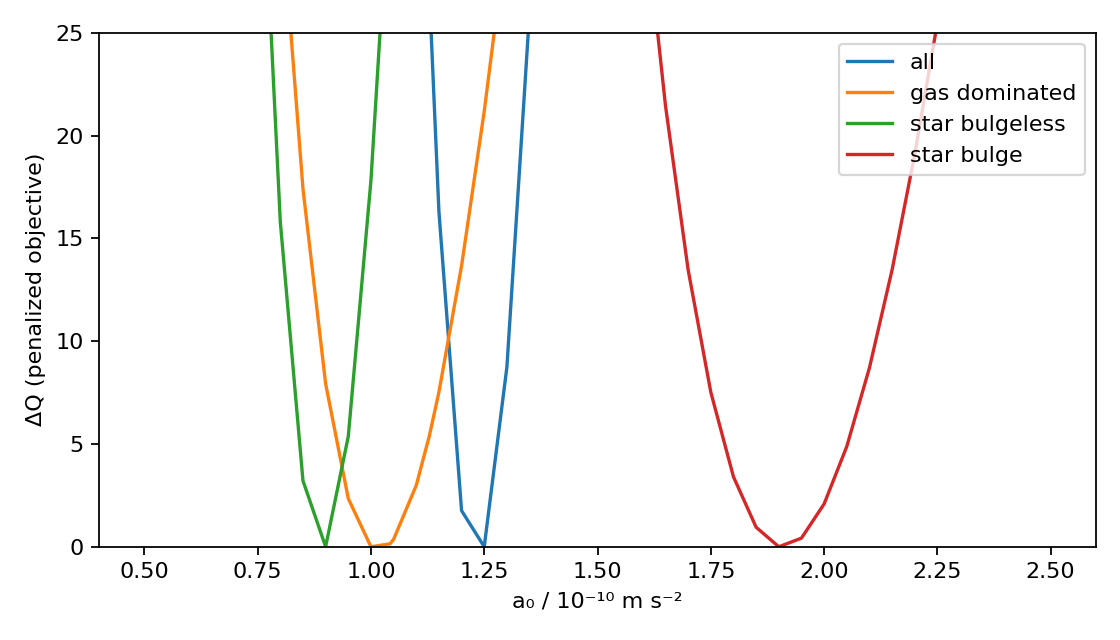
\includegraphics[width=.85\linewidth]{figures/sparc_fresh_profiles.png}
\caption{Fresh penalized objective profiles. The plotted differences are not discovery significances.}\end{figure}


\section{Bulges, systematics and interpretation}
The historical exploratory result associated a higher preferred scale with bulge-hosting galaxies. That observation motivated lighter-bulge and independently free-bulge follow-ups, which were post hoc and remain so. It would be incorrect to relabel them as prospective preregistration. A global change in bulge mass can alter the fitted disk contribution and distance/inclination, so intuition based on a single deep-limit proportionality is inadequate.

The fresh results must be interpreted under their actual fit quality. Candidate explanations include mass decomposition, distance/orientation errors, radial covariance, sample selection, noncircular motions, an inadequate interpolation law or nonuniversal dynamics. This analysis does not uniquely distinguish them. A formal contrast expressed in conditional standard errors is not a discovery significance and must not be advertised as proof of new physics.

\section{Other regimes and theoretical limits}
A separate real-data gauntlet reports S-stars, the Solar System, SPARC, SLACS, the Bullet Cluster, high-redshift disks, GW170817, Gaia wide binaries, late expansion and the CMB. Each needs an observable derived from the same named model. Data availability alone does not produce an EMRF lensing potential, tensor propagation law or cosmological perturbation spectrum. GR/CPL baselines and template agreement remain baselines, not confirmations.

Likewise, input-mass normalization in a quantum envelope is not a particle-mass prediction, and integrating an assumed $k_B/4$ per Planck area is not an independent derivation of black-hole entropy. An assigned collapse time does not predict a cosmic-dawn luminosity function. These limitations are documented separately so they cannot inflate the empirical conclusions of the SPARC paper.

\section{Correction history and reproducibility}
Earlier project releases misidentified synthetic inputs as observations and included circular tests. Their headline empirical claims are withdrawn. Subsequent stored real-data results were also described too strongly as independent verification and Bayesian marginalization. This revision distinguishes fresh computation, penalized profiling, software tests, empirical constraints and unresolved scientific questions.

The repository contains the prospective rerun protocol, raw-source manifests, versioned result artifacts, source hashes, reproducibility commands, software tests and an evidence audit. Reproducing SPARC is a re-analysis of existing observations, not independent observational replication. AI assistance was used for code and document preparation; independent expert review remains necessary. No IBM Quantum job was run and no external submission is implied.

\section{Conclusions}
The conventional acceleration scale is reproducible, but the inferred scale
depends on the sample and nuisance assumptions. The single-galaxy influence
identified in the deep-bulge subset weakens the earlier claim of a robust excess
that could establish new dynamics. Numerical reliability has improved through
explicit floor-branch optimization; observational covariance and model inadequacy
remain unresolved. These are separate uncertainties.

An acceleration-scale hypothesis can be tested without presuming a new gravitational theory. The defensible product is a transparent comparison under stated assumptions, with sensitivity and failure modes visible. Neither software pass counts nor a favorable subset establish a compression theorem, universal agreement, or novelty. Further publication decisions should follow independent review of the fresh numerical evidence and its limitations.

\bibliographystyle{plain}
\bibliography{sparc_horizon_references}
\end{document}
